\let\negmedspace\undefined
\let\negthickspace\undefined
\documentclass[journal,12pt,onecolumn]{IEEEtran}
\usepackage[margin=2.5cm]{geometry} 
\usepackage{cite}
\usepackage{amsmath,amssymb,amsfonts,amsthm}
\usepackage{algorithmic}
\usepackage{graphicx}
\graphicspath{{./figs/}}
\usepackage{textcomp}
\usepackage{xcolor}
\usepackage{txfonts}
\usepackage{listings}
\usepackage{enumitem}
\usepackage{mathtools}
\usepackage{gensymb}
\usepackage{comment}
\usepackage{caption}
\usepackage[breaklinks=true]{hyperref}
\usepackage{tkz-euclide} 
\usepackage{listings}
\usepackage{gvv}  
\usepackage{gensymb}
\usepackage{multicol}
%\def\inputGnumericTable{}                                    
\usepackage{xparse}
\usepackage{color}                                            
\usepackage{array}                                            
\usepackage{longtable}                                       
\usepackage{calc}                                             
\usepackage{multirow}
\usepackage{multicol}
\usepackage{hhline}                                           
\usepackage{ifthen}                                           
\usepackage{lscape}
\usepackage{tabularx}
\usepackage{array}
\usepackage{float}
\newtheorem{theorem}{Theorem}[section]
\newtheorem{problem}{Problem}
\newtheorem{proposition}{Proposition}[section]
\newtheorem{lemma}{Lemma}[section]
\newtheorem{corollary}[theorem]{Corollary}
\newtheorem{example}{Example}[section]
\newtheorem{definition}[problem]{Definition}
\newcommand{\BEQA}{\begin{eqnarray}}
\newcommand{\EEQA}{\end{eqnarray}}
\newcommand{\define}{\stackrel{\triangle}{=}}
\theoremstyle{remark}
\newtheorem{rem}{Remark}

\begin{document}

\title{
GATE 2023 \\
CH: CHEMICAL ENGINEERING}
\author{AI25BTECH11023 - Pratik R}
\maketitle
\renewcommand{\thefigure}{\theenumi}

\begin{enumerate}
    \item "You are delaying the completion of the task. Send \rule{40pt}{0.1mm} contributions at the
earliest."

\hfill{\brak{\text{GATE CH 2023}}}
\begin{enumerate}
    \item you are
    \item your
    \item you're
    \item yore
\end{enumerate}

    \item References : \rule{40pt}{0.1mm} : : Guidelines : Implement
    
    (By word meaning)
    
\hfill{\brak{\text{GATE CH 2023}}}
\begin{enumerate}
    \item Sight
    \item Site
    \item Cite
    \item Plagiarise
\end{enumerate}

    \item In the given figure, $PQRS$ is a parallelogram with $PS = 7 cm$, P$T = 4 cm$ and $PV = 5 cm$. What is the length of $RS$ in cm? (The diagram is representative.)
    
\hfill{\brak{\text{GATE CH 2023}}}
\begin{enumerate}
    \item $\frac{20}{7}$
    \item $\frac{28}{5}$
    \item $\frac{9}{2}$
    \item $\frac{35}{4}$
\end{enumerate}

\item In 2022, June Huh was awarded the Fields medal, which is the highest prize in
Mathematics.

When he was younger, he was also a poet. He did not win any medals in the
International Mathematics Olympiads. He dropped out of college.

Based only on the above information, which one of the following statements can be
logically inferred with certainty?

\hfill{\brak{\text{GATE CH 2023}}}
\begin{enumerate}
    \item Every Fields medalist has won a medal in an International Mathematics Olympiad.
    \item Everyone who has dropped out of college has won the Fields medal.
    \item All Fields medalists are part-time poets.
    \item Some Fields medalists have dropped out of college.
\end{enumerate}

    \item A line of symmetry is defined as a line that divides a figure into two parts in a way such that each part is a mirror image of the other part about that line.
    The given figure consists of $16$ unit squares arranged as shown. In addition to the three black squares, what is the minimum number of squares that must be coloured black, such that both $PQ$ and $MN$ form lines of symmetry? (The figure is representative)
    
\hfill{\brak{\text{GATE CH 2023}}}
%fig5

\begin{enumerate}
    \item 3
    \item 4
    \item 5
    \item 6
\end{enumerate}

    \item Human beings are the one among many creatures that inhibit an imagined world. In this imagined world, some creatures are cruel. If in this imagined world, it is given that the statement "Some human beings are not cruel creatures" is FALSE, then which of the following set of statement(s) can be logically inferred with certainty?

\begin{enumerate}[label = \roman*]
    \item All human beings are cruel creatures.
    \item some human beings are cruel creatures.
    \item Some creatures that are cruel are human beings.
    \item No human beings are cruel creatures.
\end{enumerate}

\hfill{\brak{\text{GATE CH 2023}}}
\begin{enumerate}
    \item only (i)
    \item only (iii) and (iv)
    \item only (i) and (ii)
    \item only (i), (ii) and (iii)
\end{enumerate}

    \item To construct a wall, sand and cement are mixed in the ratio of 3:1. The cost of sand and that of cement are in the ratio of 1:2.

    If the total cost sand and cement to construct wall is 1000 rupees, then what is the cost(in rupees) of cement used?
    
\hfill{\brak{\text{GATE CH 2023}}}
\begin{enumerate}
    \item 400
    \item 600
    \item 800
    \item 200
\end{enumerate}

    \item The World Bank has declared that it does not plan to offer new financing to Sri Lanka, which is battling its worst economic crisis in decades, until the country has an adequate macroeconomic policy framework in place. In a statement, the World Bank said Sri Lanka needed to adopt structural reforms that focus on economic stabilisation and tackle the root causes of its crisis. The latter has starved it of foreign exchange and led to shortages of food, fuel, and medicines. The bank is repurposing resources under existing loans to help alleviate shortages of essential items such as medicine, cooking gas, fertiliser, meals for children, and cash for vulnerable households.

    Based only on the above passage, which one of the following statements can  be inferred with certainty?
    
\hfill{\brak{\text{GATE CH 2023}}}
\begin{enumerate}
    \item According to the World Bank, the root cause of Sri Lanka’s economic crisis is that it does not have enough foreign exchange.
    \item The World Bank has stated that it will advise the Sri Lankan government about how to tackle the root causes of its economic crisis.
    \item According to the World Bank, Sri Lanka does not yet have an adequate macroeconomic policy framework.
    \item The World Bank has stated that it will provide Sri Lanka with additional funds for essentials such as food, fuel, and medicines.
\end{enumerate}
\newpage
    \item The coefficient of $x^4$ in the polynomial$ \brak{x - 1}^3\brak{x - 2}^3$ is equal to \rule{40pt}{0.1mm}.
    
\hfill{\brak{\text{GATE CH 2023}}}
\begin{enumerate}
    \item 33
    \item -3
    \item 30
    \item 21
\end{enumerate}

    \item Which one of the following shapes can be used to tile (completely cover by repeating) a flat plane, extending to infinity in all directions, without leaving any empty spaces in between them? The copies of the shape used to tile are identical and are not allowed to overlap.
    
\hfill{\brak{\text{GATE CH 2023}}}
\begin{enumerate}
    \item circle 
    \item regular octagon 
    \item regular pentagon
    \item rhombus
\end{enumerate}

    \item Which of the following is the CORRECT value of y, as defined by the expression given below?

    \begin{align*}
        y = \lim_{x\to 0} \frac{2x}{e^x - 1}
    \end{align*}
    
\hfill{\brak{\text{GATE CH 2023}}}
\begin{enumerate}
    \item 1
    \item 2
    \item 0
    \item $\infty$
\end{enumerate}

    \item The vector $\vec v$ is defined as 
    
    \begin{align*}
        \vec v = zx \hat{i} + 2xy \hat{j} + 3yz \hat{k}
    \end{align*} 

    Which of the following is the CORRECT value of divergence of $\vec v$, evaluated at the point $(x,y,z) = (3,2,1)$?

\hfill{\brak{\text{GATE CH 2023}}}
\begin{enumerate}
    \item 0
    \item 3
    \item 14
    \item 13
\end{enumerate}
\newpage
    \item Given that 

    \begin{align*}
      F = \frac{|z_1 + z_2|}{|z_1| + |z_2|}
    \end{align*}

    where $z_1 = 2 + 3i$ and $z_2 = -2 + 3i$ with $i = \sqrt{-1}$, which of the following options is CORRECT?
    
\hfill{\brak{\text{GATE CH 2023}}}
\begin{enumerate}
    \item $F < 0$
    \item $F < 1$
    \item $F > 1$
    \item $F = 1$
\end{enumerate}

    \item For a two-dimensional plane, the unit vectors, $\brak{\hat{e}_{r}, \hat{e}_{\theta}}$ of the polar coordinate system and $\brak{\hat{i}, \hat{j}}$ of the cartesian coordinate system, are related by the following two equations.

    \begin{align*}
        \hat{e}_{r} &= cos\theta \hat{i} + sin\theta \hat{j} \\
        \hat{e}_{\theta} &= -sin\theta \hat{i} + cos\theta \hat{j}
    \end{align*}

    Which of the following is the CORRECT value of $\frac{\partial \brak{\hat{e}_{r} + \hat{e}_{\theta}}}{\partial \theta}$ ?
    
\hfill{\brak{\text{GATE CH 2023}}}
\begin{enumerate}
    \item 1
    \item $\hat{e}_{\theta}$
    \item $\hat{e}_{r} + \hat{e}_{\theta}$
    \item $-\hat{e}_{r} + \hat{e}_{\theta}$
\end{enumerate}

    \item Which one of the following statements related to octane number is NOT correct?
    
\hfill{\brak{\text{GATE CH 2023}}}
\begin{enumerate}
    \item Linear alkanes with higher carbon number have higher octane number.
    \item Branching in linear alkanes increases their octane number.
    \item Catalytic reforming of hydrocarbons increases their octane number.
    \item Gasoline quality is measured in terms of octane number.
\end{enumerate}

    \item Which one of the following options represents the major components of oleum?
    
\hfill{\brak{\text{GATE CH 2023}}}
\begin{enumerate}
    \item Sulfuric acid and nitric acid
    \item Concentrated sulfuric acid and petroleum jelly
    \item Sulfuric acid and hydrochloric acid
    \item Sulfuric acid and sulfur trioxide
\end{enumerate}
\newpage
    \item For a reversible endothermic chemical reaction with constant heat of reaction over the operating temperature range, $K$ is the thermodynamic equilibrium constant. Which one of the following figures shows the CORRECT dependence of $K$ on temperature $T$?
    
\hfill{\brak{\text{GATE CH 2023}}}
\begin{multicols}{2}
    \begin{enumerate}
        \item \begin{figure}[H]
            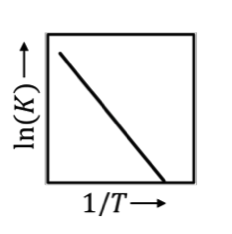
\includegraphics[width=0.25\linewidth]{figs/17a.png}
            \label{fig:17a}
        \end{figure}
        \item \begin{figure}[H]
            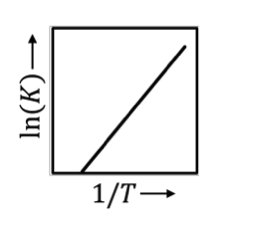
\includegraphics[width=0.25\linewidth]{figs/17b.png}
            \label{fig:17b}
        \end{figure}
        \item \begin{figure}[H]
            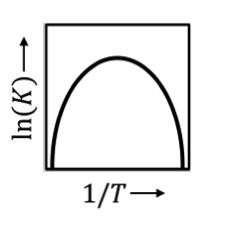
\includegraphics[width=0.25\linewidth]{figs/17c.png}
            \label{fig:17c}
        \end{figure}
        \item \begin{figure}[H]
            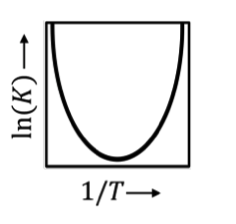
\includegraphics[width=0.25\linewidth]{figs/17d.png}
            \label{fig:17d}
        \end{figure}
    \end{enumerate}
\end{multicols}
    \item Nitrile rubber is manufactured via polymerization process. Which one of the following options is the CORRECT pair of monomers used in this process?
    
\hfill{\brak{\text{GATE CH 2023}}}
\begin{enumerate}
    \item Acrylonitrile and styrene
    \item Acrylonitrile and butadiene
    \item Butadiene and styrene
    \item Butadiene and isoprene
\end{enumerate}

    \item John and Jane independently performed a thermodynamic experiment, in which \textbf{X} and \textbf{Y} represent the initial and final thermodynamic states of the system, respectively. John performed the experiment under reversible conditions, for which the change in entropy of the system was $\Delta S_{rev}$ . Jane performed the experiment under irreversible conditions, for which the change in entropy of the system was $\Delta S_{irr}$ . Which one of the following relationships is CORRECT?
    
\hfill{\brak{\text{GATE CH 2023}}}
\begin{enumerate}
    \item $\Delta S_{rev} = \Delta S_{irr}$
    \item $\Delta S_{rev} > \Delta S_{irr}$
    \item $\Delta S_{rev} < \Delta S_{irr}$
    \item $\Delta S_{rev} = 2\Delta S_{irr}$
\end{enumerate}

     \item For a packed-bed comprising of uniform-sized spherical particles of diameter $D_p$, the pressure drop across the bed is given by the Kozeny-Carman equation when the particle Reynolds number $\brak{Re_p} < 1$. Under this condition, minimum fluidization velocity is proportional to $D^n_p$. Which one of the following is the CORRECT value of exponent $n$ ?
     
\hfill{\brak{\text{GATE CH 2023}}}
\begin{enumerate}
    \item 2
    \item -1
    \item -2
    \item 1
\end{enumerate}

    \item Match the quantities in Group 1 with their units in Group 2 listed in the table below.
    
\hfill{\brak{\text{GATE CH 2023}}}
\begin{multicols}{2}
    \begin{enumerate}[label = \Alph*]
        \item Thermal conductivity
        \item Convective heat transfer coefficient 
        \item Stefan-Boltzmann constant 
        \item Heat capacity rate 
    \end{enumerate}

\columnbreak

\begin{enumerate}[label = \Roman*]
    \item $W\cdot m^{-2}K^{-1}$
    \item $W\cdot m^{-1}K^{-1}$
    \item $W\cdot K^{-1}$
    \item $W\cdot m^{-2}K^{-4}$
\end{enumerate}
\end{multicols}

\begin{enumerate}
    \item A-II, B-I, C-IV, D-III
    \item A-I, B-II, C-III, D-IV
    \item A-III, B-IV, C-II, D-I
    \item A-IV, B-I, C-III, D-II
\end{enumerate}

    \item A slab of thickness $L$, as shown in the figure below, has cross-sectional area $A$ and constant thermal conductivity $k$. $T_1$ and $T_2$ are the temperatures at $x = 0$ and $x = L$, respectively. Which one of the following options is the CORRECT expression of the thermal resistance for steady-state one-dimensional heat conduction?

\hfill{\brak{\text{GATE CH 2023}}}

%fig22

\begin{enumerate}
    \item $\frac{L}{kA}$
    \item $\frac{k}{LA}$
    \item $\frac{kA\brak{T_1 - T_2}}{L}$
    \item $\frac{A}{Lk}$
\end{enumerate}

    \item Spray dryers have many advantages. Which one of the following is NOT an advantage of a typical spray dryer

\hfill{\brak{\text{GATE CH 2023}}}
\begin{enumerate}
    \item Has short drying time
    \item Produces hollow spherical particles
    \item Has high heat efficiency
    \item Is suitable for heat sensitive materials
\end{enumerate}

    \item Which one of the following quantities of a flowing fluid is measured using a rotameter?

\hfill{\brak{\text{GATE CH 2023}}}
\begin{enumerate}
    \item Static pressure
    \item Dynamic pressure
    \item Volumetric flow rate
    \item Viscosity
\end{enumerate}

    \item A liquid surge tank has $F_{in}$ and $F_{out}$ as the inlet and outlet flow rates respectively, as shown in the figure below. $F_out$ is proportional to the square root of the liquid level $h$. The cross-sectional area of the tank is $20cm^{2}$. Density of the liquid is constant everywhere in the system. At steady state,$F_{in} = F_{out} = 10cm^{3}s^{-1}$ and $h = 16cm$. The variation of $h$ with $F_{in}$ is approximated as a first order transfer function. Which one of the following is the CORRECT value of the time constant (in seconds) of this system?

\hfill{\brak{\text{GATE CH 2023}}}
%fig25

\begin{enumerate}
    \item 20
    \item 32
    \item 64
    \item 128
\end{enumerate}

    \item A packed distillation column, with vapor having an average molecular weight of $45 kg\cdot kmol^{-1}$, density of $2kg\cdot m^{-3}$ and a molar flow rate of $0.1 kmol\cdot s^{-1}$, has a flooding velocity of $0.15m\cdot s^{-1}$. The column is designed to operate at 60\% of the flooding velocity. Which one of the following is the CORRECT value for the column diameter (in m)?
    
\hfill{\brak{\text{GATE CH 2023}}}
\begin{enumerate}
    \item $\frac{5}{\sqrt{\pi}}$
    \item $5\sqrt{\pi}$
    \item $4\pi$
    \item $\frac{10}{\sqrt{\pi}}$
\end{enumerate}

    \item An isothermal jacketed continuous stirred tank reactor (CSTR) operating at $150^{o}C$ is shown in the figure below. The cold feed entering the system at $30^oC$ is preheated to a temperature $T\brak{T < 150^oC}$ using a heat exchanger $HX_1$. This preheated feed is further heated to $150^oC$ using the utility heater $HX_2$. The mass flow rate and heat capacity are same for all the process streams, and the overall heat transfer coefficient is independent of temperature. Which one of the following statements is the CORRECT action to take if it is desired to increase the value of $T$ ?

\hfill{\brak{\text{GATE CH 2023}}}
\begin{figure}[H]
    \centering
    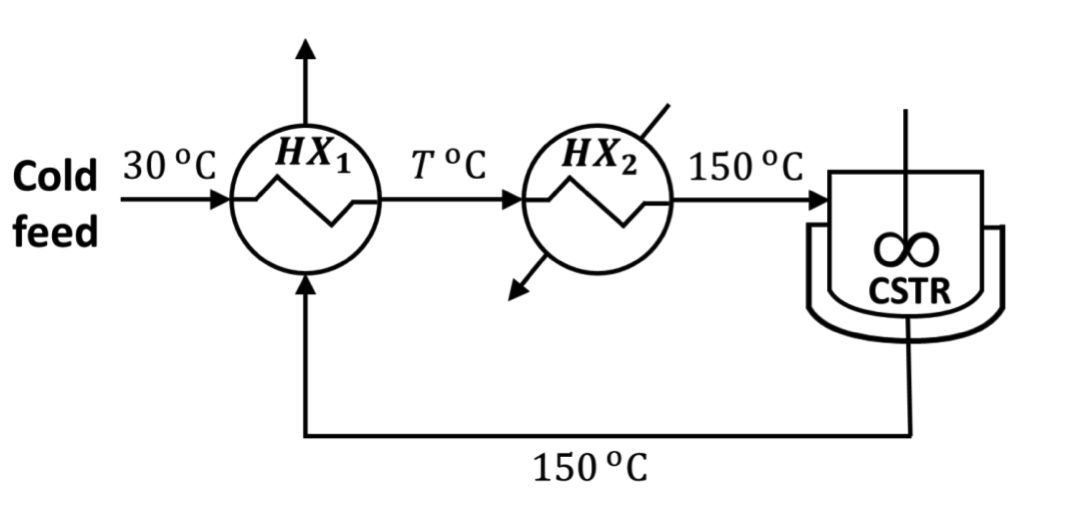
\includegraphics[width=0.8\columnwidth]{figs/27.png}
    \caption{}
    \label{fig:27}
\end{figure}

\begin{enumerate}
    \item Increase both heat transfer area of $HX_1$ and heat duty of $HX_2$.
    \item Decrease both heat transfer area of $HX_1$ and heat duty of $HX_2$.
    \item Increase the heat transfer area of $HX_1$ and decrease the heat duty of $HX_2$
    \item Decrease the heat transfer area of $HX_1$ and increase the heat duty of $HX_2$2.
\end{enumerate}

    \item Consider a system where a Carnot engine is operating between a source and a sink. Which of the following statements about this system is/are NOT correct?

\hfill{\brak{\text{GATE CH 2023}}}
\begin{enumerate}
    \item This engine is reversible.
    \item The engine efficiency is independent of the source and sink temperatures.
    \item This engine has the highest efficiency among all engines that operate between the same source and sink.
    \item The total entropy of this system increases at the completion of each cycle of the engine.
\end{enumerate}

    \item For a fully developed turbulent flow of an incompressible Newtonian fluid through a pipe of constant diameter, which of the following statements is/are CORRECT?

\hfill{\brak{\text{GATE CH 2023}}}
\begin{enumerate}
    \item Reynolds stress, averaged over a sufficiently long time, is zero everywhere inside the pipe.
    \item Reynolds stress at the pipe wall is zero.
    \item Average velocity of the fluid is half of its center-line velocity.
    \item Average pressure gradient in the flow direction is constant.
\end{enumerate}

    \item Given that $E\brak{in W\cdot m^{-2}}$ is the total hemispherical emissive power of a surface maintained at a certain temperature, which of the following statements is/are CORRECT?

\hfill{\brak{\text{GATE CH 2023}}}
\begin{enumerate}
    \item $E$ does not depend on the direction of the emission.
    \item $E$ depends on the viewfactor.
    \item $E$ depends on the wavelength of the emission.
    \item $E$ does not depend on the frequency of the emission.
\end{enumerate}

    \item The position $x\brak{t}$ of a particle, at constant $\omega$, is described by the equation

    \begin{align*}
        \frac{d^{2}x}{dt^{2}} = -w^2x
    \end{align*}

    The initial conditions are $x\brak{t = 0} = 1$ and $\frac{dx}{dt}|_{t=0} = 0$. The position of the particle at $t = \brak{\frac{3\pi}{\omega}}$ is \rule{40pt}{0.1mm} (in integer).

\hfill{\brak{\text{GATE CH 2023}}}
    \item Burning of methane in a combustor yields carbon monoxide, carbon dioxide, and water vapor. Methane is fed to the combustor at $100 mol\cdot hr^{-1}$, of which 50 \% reacts. The theoretical oxygen requirement (in $mol\cdot hr^{-1}$) is \rule{40pt}{0.1mm} (rounded off to one decimal place).

\hfill{\brak{\text{GATE CH 2023}}}
    \item The viscosity of an incompressible Newtonian fluid is measured using a capillary tube of diameter 0.5 mm and length 1.5 m. The fluid flow is laminar, steady and fully developed. For a flow rate of $1cm^3s^{-1}$, the pressure drop across the length of the tube is $1MPa$. If the viscosity of the fluid is $k\times 10^{-3}Pa.s$, the value of $k$ is \rule{40pt}{0.1mm} (rounded off to two decimal places).

\hfill{\brak{\text{GATE CH 2023}}}
    \item A liquid $L$ containing a dissolved gas $S$ is stripped in a countercurrent operation
    using a pure carrier gas $V$. The liquid phase inlet and outlet mole fractions of $S$ are
    0.1 and 0.01, respectively. The equilibrium distribution of $S$ between $V$ and $L$ is
    governed by $y_e = x_e$, where $y_e$ and $x_e$ are the mole fractions of $S$ in $V$ and $L$,
    respectively. The molar feed rate of the carrier gas stream is twice as that of the liquid
    stream. Under dilute solution conditions, the minimum number of ideal stages required is \rule{40pt}{0.1mm} (in integer).

    \hfill{\brak{\text{GATE CH 2023}}}
    \item In a binary gas-liquid system, $N_{A,EMD}$ is the molar flux of a gas $A$ for equimolar
    counter diffusion with a liquid $B$. $N_{A,UMD}$ is the molar flux of $A$ for steady one-component
    diffusion through stagnant $B$. Using the mole fraction of $A$ in the bulk of the gas phase
    as 0.2 and that at the gas-liquid interface as 0.1 for both the modes of diffusion, the ratio of
    $N_{A,UMD}$ to $N_{A,EMD}$ is equal to \rule{40pt}{0.1mm} (rounded off to two decimal places).

    \hfill{\brak{\text{GATE CH 2023}}}
    \item An exhibition was held in a hall on 15 August 2022 between 3 PM and 4 PM during
    which any person was allowed to enter only once. Visitors who entered before 3:40 PM exited exactly after 20 minutes from their time of entry.
    Visitors who entered at or after 3:40 PM exited exactly at 4 PM. The probability distribution of the arrival time of any visitor is uniform between 3 PM and 4 PM. Two persons $X$ and $Y$ entered the exhibition hall independent of each other. Which one of the following values is the probability that their visits to the exhibition overlapped with each other?

    \hfill{\brak{\text{GATE CH 2023}}}
    \begin{enumerate}
        \item $\frac{5}{9}$
        \item $\frac{4}{9}$
        \item $\frac{2}{9}$
        \item $\frac{7}{9}$
    \end{enumerate}
    
    \item Simpson’s one-third rule is used to estimate the definite integral
    \begin{align*}
        I = \int_{-1}^{1} \sqrt{1-x^2} \, dx
    \end{align*}
    
    with an interval length of $0.5$. Which of the following is the correct estimate of $I$ using this rule?
    
    \hfill{\brak{\text{GATE CH 2023}}}
    \begin{enumerate}
        \item $\frac{1}{3} - \frac{1}{\sqrt{3}}$
        \item $\frac{1}{3} + \frac{2}{\sqrt{3}}$
        \item $\frac{1}{3} + \frac{1}{\sqrt{3}}$
        \item $\frac{1}{3} - \frac{2}{\sqrt{3}}$
    \end{enumerate}

    \item Match the products in Group 1 with the manufacturing processes in Group 2 listed in the table below.

    \hfill{\brak{\text{GATE CH 2023}}}
    \begin{multicols}{2}
    \begin{enumerate}[label=\Alph*]
        \item Acetaldehyde
        \item Sulfuric acid
        \item Pulp
        \item Phosphorus
    \end{enumerate}
    \columnbreak
    \begin{enumerate}[label=\Roman*]
        \item Sulfate process
        \item Electric furnace process
        \item Wacker process
        \item Contact process
    \end{enumerate}
    \end{multicols}
    \begin{enumerate}
        \item A-III, B-IV, C-I, D-II
        \item A-III, B-I, C-IV, D-II
        \item A-IV, B-I, C-II, D-III
        \item A-I, B-IV, C-II, D-III
    \end{enumerate}
\newpage
    \item Match the reactions in Group 1 with the catalysts in Group 2:

    \hfill{\brak{\text{GATE CH 2023}}}
    \begin{table}[H]
\centering
\begin{tabularx}{0.8\textwidth}{|l|X|}
\hline
\textbf{Group 1} & \textbf{Group 2} \\
\hline
P) $C_6H_6 + Cl_2 \to Chlorobenzene + HCl$ & I) Mixed oxide of Mo and Fe \\
\hline
Q) $H_2C = CH_2 + \frac{1}{2}0_2 \to Ethylene oxide$ & II) $V_2O_5$ \\
\hline
R) $CH_3OH + \frac{1}{2}O_2 \to Formaldehyde + H_2O$ & III) $FeCl_3$ \\
\hline
S) $Naphthalene + \frac{9}{2} O_2 \to Phthalic anhydride + 2H_2O + 2CO_2$ & IV) $Ag_2O$ \\
\hline 
\end{tabularx}
\caption*{}
\label{tables:59}
\end{table}
    \begin{enumerate}
        \item P-III, Q-IV, R-II, S-I
        \item P-III, Q-IV, R-I, S-II
        \item P-IV, Q-II, R-I, S-III
        \item P-IV, Q-III, R-I, S-II
    \end{enumerate}

    \item Water in a container at$290 K$ is exposed to air containing 3 \% $CO_2$ by volume. Air behaves like an ideal gas and is maintained at $100 kPa$ pressure. The liquid phase comprising of dissolved $CO_2$ in water behaves like an ideal solution. Use Henry’s constant of $CO_2$ dissolved in water at $290 K$ as $12 MPa$. Under equilibrium conditions, which one of the following is the CORRECT value of the mole fraction of $CO_2$ dissolved in water?

    \hfill{\brak{\text{GATE CH 2023}}}
    \begin{enumerate}
        \item $2.9 \times 10^{-4}$
        \item $0.9 \times 10^{-4}$
        \item $2.5 \times 10^{-4}$
        \item $0.5 \times 10^{-4}$
    \end{enumerate}

    \item The enthalpy ($H, j\cdot mol^{-1}$) of a binary liquid system at constant temperature and pressure is given as
    \begin{align*}
        H = 40x_1 + 60x_2 + x_1x_2\brak{4x_1 + 2x_2}
    \end{align*}
    where $x_1$ and $x_2$ represent the mole fractions of species 1 and 2 in the liquid, respectively. Which one of the following is the CORRECT value of the partial molar enthalpy of species 1 at infinite dilution, $\Bar{H}_{1}$ in ($J\cdot mol^{-1}$)?

    \hfill{\brak{\text{GATE CH 2023}}}
    \begin{enumerate}
        \item 100
        \item 42
        \item 64
        \item 40
    \end{enumerate}

    \item Which one of the following represents the CORRECT effects of concentration polarization in a reverse osmosis process?

    \hfill{\brak{\text{GATE CH 2023}}}
    \begin{enumerate}
        \item Reduced water flux and reduced solute rejection
        \item Increased water flux and increased solute rejection
        \item Reduced water flux and increased solute rejection
        \item Increased water flux and reduced solute rejection
    \end{enumerate}
    \newpage
   \item CO and H2 participate in a catalytic reaction. The partial pressures (in atm) of the reacting species CO and H2 in the feed stream are $p_{CO}$ and $p_{H_2}$, respectively. While CO undergoes molecular adsorption, $H_2$ adsorbs via dissociative adsorption, that is, as hydrogen atoms. The equilibrium constants (in $atm^{-1}$) corresponding to adsorption of CO and $H_2$ to the catalyst sites are $K_{CO}$ and $K_{H_2}$, respectively. Total molar concentration of active sites per unit mass of the catalyst is $C_t$ (in $mol\cdot \brak{g cat}^{-1}$). Both the adsorption steps are at equilibrium. Which one of the following expressions is the CORRECT ratio of the concentration of catalyst sites occupied by CO to that by hydrogen atoms?

\hfill{\brak{\text{GATE CH 2023}}}
   \begin{enumerate}
       \item $\frac{K_{CO}p_{CO}}{\sqrt{K_{H_2}p_{H_2}}}$
       \item $\frac{K_{CO}}{\sqrt{K_{H_2}}}$
       \item $\frac{p_{CO}}{\sqrt{p_{H_2}}}$
       \item $\frac{K_{CO}p_{CO}}{K_{H_2}p_{H_2}}$
   \end{enumerate}
   
    \item A cascade control strategy is shown in the figure below. The transfer function between the output $\brak{y}$ and the secondary disturbance $\brak{d_2}$) is defined as
    \begin{align*}
        G_{d2}\brak{s} = \frac{y\brak{s}}{d_2\brak{s}}
    \end{align*}
    Which one of the following is the CORRECT expression for the transfer function $G_{d2}\brak{s}$ ?
    
    \hfill{\brak{\text{GATE CH 2023}}}
    \begin{figure}[H]
        \centering
        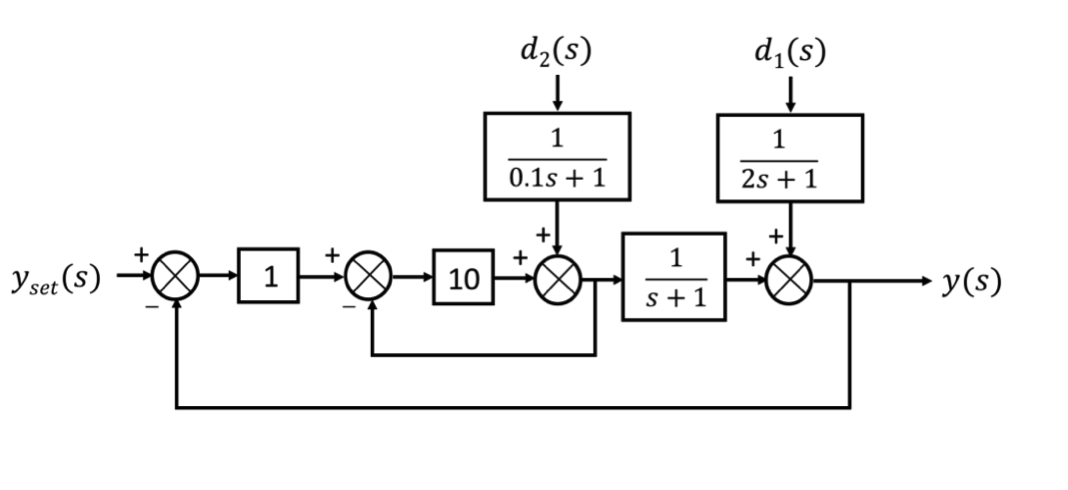
\includegraphics[width=0.8\columnwidth]{figs/44.png}
        \caption{}
        \label{fig:44}
    \end{figure}
    \begin{enumerate}
        \item $\frac{1}{\brak{11s+21}\brak{0.1s+1}}$
        \item $\frac{1}{\brak{s+1}\brak{0.1s+1}}$
        \item $\frac{s+1}{\brak{s+2}\brak{0.1s+1}}$
        \item $\frac{s+1}{\brak{s+1}\brak{0.1s+1}}$
    \end{enumerate}
    \newpage
    \item Level $\brak{h}$ in a steam boiler is controlled by manipulating the flow rate $\brak{F}$ of the make-up (fresh) water using a proportional $\brak{P}$ controller. The transfer function between the output and the manipulated input is 

    \begin{align*}
        \frac{h\brak{s}}{F\brak{s}} = \frac{0.25\brak{1-s}}{s\brak{2s+1}}  
    \end{align*}
    The measurement and valve transfer functions are both equal to 1. A process engineer wants to tune the controller so that the closed-loop response gives decaying oscillations under servo mode. Which one of the following is the CORRECT value of the controller gain to be used by the engineer?

    \hfill{\brak{\text{GATE CH 2023}}}
    \begin{enumerate}
        \item 0.25
        \item 2
        \item 4
        \item 6
    \end{enumerate}
    
    \item Which of the following statements is/are CORRECT?

    \hfill{\brak{\text{GATE CH 2023}}}
    \begin{enumerate}
        \item Bond number includes surface tension
        \item Jakob number includes latent heat
        \item Prandtl number includes liquid-vapor density difference
        \item Biot number includes gravity
    \end{enumerate}

    \item If a matrix $M$ is defined as $M =\myvec{
    10 & 6 \\
    6 & 10 \\
    }$, the sum of all the eigenvalues of $M^3$ is
equal to \rule{40pt}{0.1mm} (in integer).

    \hfill{\brak{\text{GATE CH 2023}}}
    \item The first derivative of the function
    \begin{align*}
        U\brak{r} = 4\sbrak{\brak{\frac{1}{r}}^{12} - \brak{\frac{1}{r}}^{6}} 
    \end{align*}
    evaluated at $r=1$ is \rule{40pt}{0.1mm} (in integer)

\hfill{\brak{\text{GATE CH 2023}}}
    \item Wet air containing 10 mole percent water vapor is dried by continuously passing it through a column of $CaCl_2$ pellets. The pellets remove 50 percent of water from wet air entering the column. The mole percent of water vapor in the product stream exiting the column is \rule{40pt}{0.1mm}(rounded off to two decimal places).

    \hfill{\brak{\text{GATE CH 2023}}}
    \item Orsat analysis showing the composition (in mol \%, on a dry basis) of a stack gas is given in the table below. The humidity measurement reveals that the mole fraction of $H_2O$ in the stack gas is $0.07$. The mole fraction of $N_2$ calculated on a wet basis is \rule{40pt}{0.1mm}(rounded off to two decimal places).

    \hfill{\brak{\text{GATE CH 2023}}}
    \begin{table}[H]
\centering
\begin{tabularx}{0.4\textwidth}{|l|X|X|X|X|}
\hline
\textbf{Species} & $N_2$ & $CO_2$ & $CO$ & $O_2$  \\
\hline
\textbf{mol\%} & 65 & 15 & 10 & 10 \\
\hline
\end{tabularx}
\caption*{}
\label{tables:59}
\end{table}
    \item A pump draws water ($density = 1000 kg\cdot m^{-3}$) at a steady rate of $10 kg\cdot s^{-1}$. The pressures at the suction and discharge sides of the pump are $-20 kPa$ (gauge) and $350 kPa$ (gauge), respectively. The pipe diameters at the suction and discharge side are $70 mm$ and $50 mm$, respectively. The suction and discharge lines are at the same elevation, and the pump operates at an efficiency of 80 \%. Neglecting frictional losses in the system, the power (in kW) required to drive the pump is \rule{40pt}{0.1mm}(rounded off to two decimal places).

    \hfill{\brak{\text{GATE CH 2023}}}
    \item A cylindrical tank with a diameter of 500 mm contains water $\brak{density = 1 g.cm^{-3}}$ upto a height $h$. A 5 mm diameter round nozzle, whose center is 1 cm above the base of the tank, has its exit open to the atmosphere as shown in the schematic below. The pressure above the water level in the tank is maintained at 2 bar (absolute). Neglect all frictional and entry/exit losses. Use acceleration due to gravity as $10 ms^{-2}$ and atmospheric pressure as 1 bar. The absolute value of initial $\frac{dh}{dt}\brak{mm\cdot s^{-1}}$ when $h = 51 cm$ is equal to \rule{40pt}{0.1mm}(rounded off to two decimal places).

    \hfill{\brak{\text{GATE CH 2023}}}
    \begin{figure}[H]
        \centering
        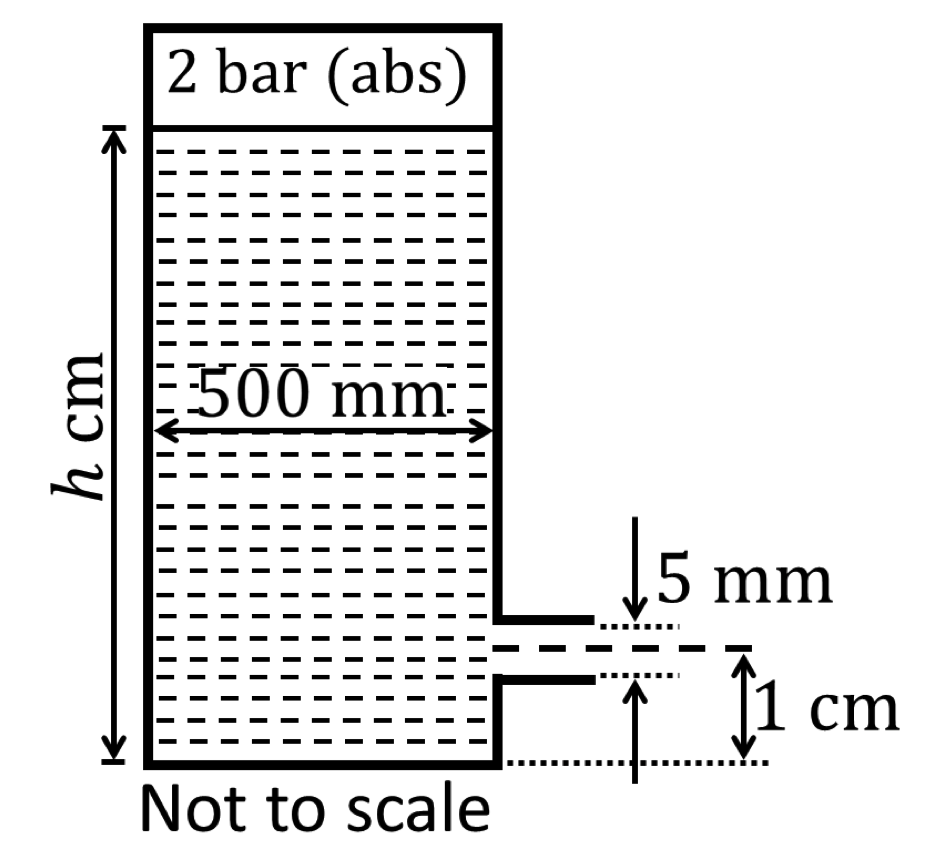
\includegraphics[width=0.5\columnwidth]{figs/52.png}
        \caption{}
        \label{fig:52}
    \end{figure}
    \item A large tank is filled with water $\brak{density = 1 g.cm^{-3}}$ upto a height of $5m$. A $100 \mu m$ diameter solid spherical particle $\brak{density = 0.8 g.cm^{-3}}$ is released at the bottom of the tank. The particle attains its terminal velocity $\brak{v_t}$ after traveling to a certain height in the tank. Use acceleration due to gravity as $10 ms^{-2}$ and water viscosity as $10^{-3}Pa\cdot s$ . Neglect wall effects on the particle. If Stokes law is applicable, the absolute value of $v_t\brak{in mm\cdot s^{-1}}$ is \rule{40pt}{0.1mm}(rounded off to two decimal places).

    \hfill{\brak{\text{GATE CH 2023}}}
\newpage
    \item A fluid is flowing steadily under laminar conditions over a thin rectangular plate at temperature $T_s$ as shown in the figure below. The velocity and temperature of the free stream are $u_{\infty}$ and $T_{\infty}$, respectively. When the fluid flow is only in the $x$ direction, $h_x$ is the local heat transfer coefficient. Similarly, when the fluid flow is only in the $y$ direction, $h_y$ is the corresponding local heat transfer coefficient. Use the correlation $Nu = 0.332(Re)^{1/2} (Pr )^{1/3}$ for the local heat transfer coefficient, where, $Nu$, $Re$, and $Pr$, respectively are the appropriate Nusselt, Reynolds and Prandtl numbers. The average heat transfer coefficients are defined as
    $\Bar{h}_l = \frac{1}{l} \int_{0}^{l} h_x \,dx$ and $\Bar{h}_w = \frac{1}{w} \int_{0}^{w} h_y \,dy$. if $w = 1m$ and $l = 4m$, the value of the ratio of $\Bar{h}_w$ to $\Bar{h}_l$ is \rule{40pt}{0.1mm}(in integer).

    \hfill{\brak{\text{GATE CH 2023}}}
\begin{figure}[H]
    \centering
    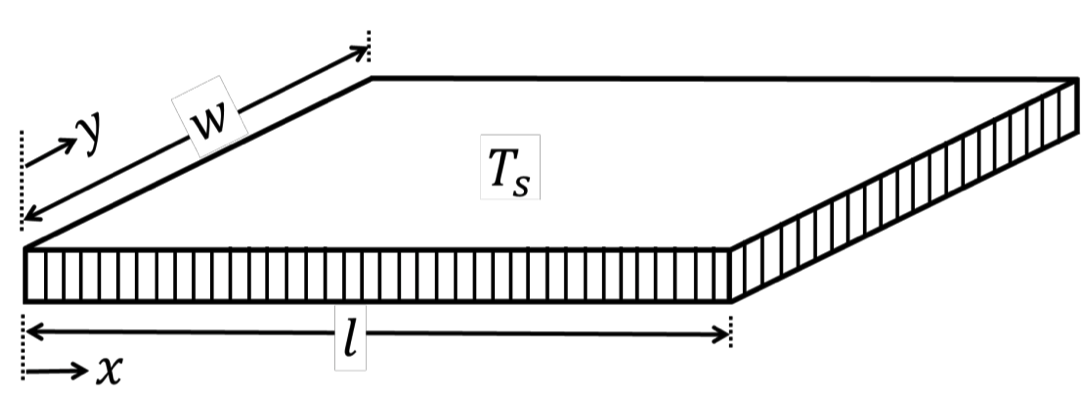
\includegraphics[width=0.5\columnwidth]{figs/54.png}
    \caption{}
    \label{fig:54}
\end{figure}
    \item A perfectly insulated, concentric tube countercurrent heat exchanger is used to cool lubricating oil using water as a coolant (see figure below). Oil enters the outer annulus at a mass flow rate of $2kg\cdot s^{-1}$ with a temperature of $100^oC$ and leaves at $40^oC$. Water enters the inner tube at a mass flow rate of $1kg\cdot s^{-1}$ with a temperature of $20^oC$ and leaves at $80^oC$. Use specific heats of oil and water as $2089 J\cdot kg^{-1}K^{-1}$ and $4178 J\cdot kg^{-1}K^{-1}$, respectively. There is no phase change in both the streams. Under steadystate conditions, the number of transfer units (NTU) is \rule{40pt}{0.1mm} (in integer).

    \hfill{\brak{\text{GATE CH 2023}}}
    \begin{figure}[H]
        \centering
        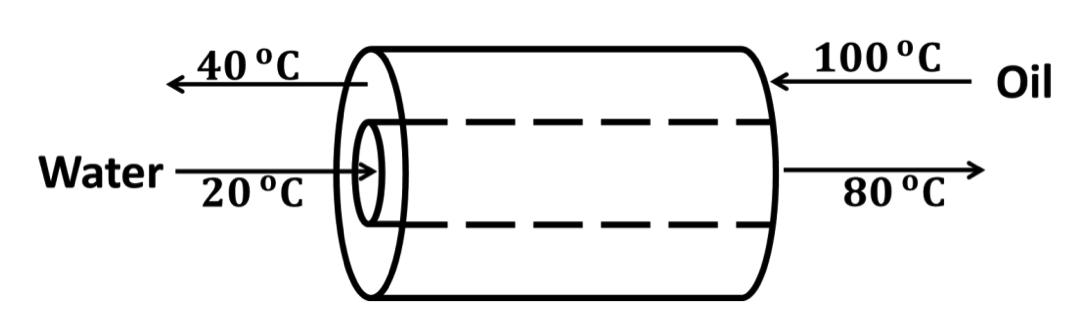
\includegraphics[width=0.5\columnwidth]{figs/55.png}
        \caption{}
        \label{fig:55}
    \end{figure}
    \item Partially saturated air at 1 bar and $50\degree C$ is contacted with water in an adiabatic saturator. The air is cooled and humidified to saturation, and exits at $25\degree C$ with an absolute humidity of $0.02 kg$ water per kg dry air. Use latent heat of vaporization of water as $2450 kJ\cdot kg^{-1}$, and average specific heat capacity for dry air and water, respectively as $1.01 kJ\cdot kg^{-1}K^{-1}$ and $4.18 kJ\cdot kg^{-1}K^{-1}$. If the absolute humidity of air entering the adiabatic saturator is $H\times 10^{-3} kg$ water per kg dry air, the value of $H$ is \rule{40pt}{0.1mm}(rounded off to two decimal places).

    \hfill{\brak{\text{GATE CH 2023}}}
\newpage
    \item Distillation of a non-reactive binary mixture with components $A$ and $B$ is carried out in a batch still as shown in the figure below. The initial charge of the mixture in the still is $1 kmol$. The initial and final amounts of $A$ in the still are $0.1 kmol$ and $0.01 kmol$, respectively. Use a constant relative volatility of $4.5$. The mole fraction of $B$ remaining in the vessel is \rule{40pt}{0.1mm} (rounded off to three decimal places).

    \hfill{\brak{\text{GATE CH 2023}}}
\begin{figure}[H]
    \centering
    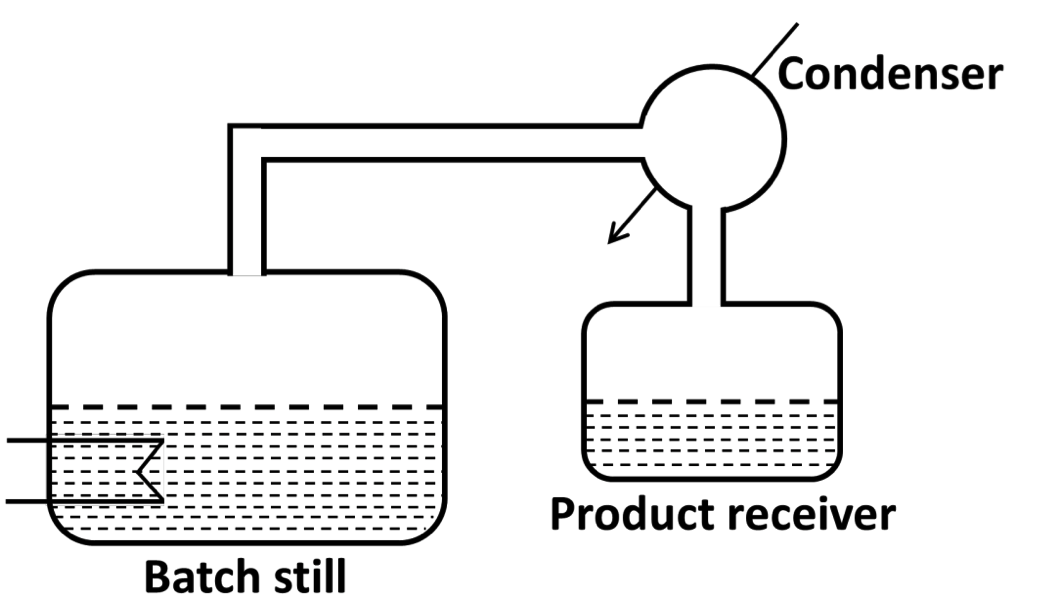
\includegraphics[width=0.5\columnwidth]{figs/57.png}
    \caption{}
    \label{fig:57}
\end{figure}
    \item Fresh catalyst is loaded into a reactor before the start of the following catalytic reaction.
    \begin{align*}
        A \to products
    \end{align*}
    The catalyst gets deactivated over time. The instantaneous activity $\alpha \brak{t}$, at time $t$, is defined as the ratio of the rate of reaction $-r'_A\brak{t}\brak{mol\cdot \brak{gcat}^{-1}hr^{-1}}$ to the rate of reaction with fresh catalyst. Controlled experimental measurements led to an empirical correlation
    \begin{align*}
        -r'_A\brak{t} = -0.5t + 10
    \end{align*}
    where $t$ is in hours. The activity of the catalyst at $t = 10hr$ is \rule{40pt}{0.1mm} (rounded off to one decimal place).

    \hfill{\brak{\text{GATE CH 2023}}}
    \item A unimolecular, irreversible liquid-phase reaction
    \begin{align*}
        A \to P
    \end{align*}
    was carried out in an ideal batch reactor at temperature $T$. The rate of the reaction $\brak{-r_A}$ measured at different conversions $X_A$ is given in the table below. This reaction is also carried out in an ideal continuous stirred tank reactor (CSTR) at the same temperature $T$ with a feed concentration of $1mol\cdot m^{-3}$, under steady-state conditions. For a conversion of $0.8$, the space time (in s) of the CSTR is \rule{40pt}{0.1mm}(in integer).
    
    \hfill{\brak{\text{GATE CH 2023}}}

    \begin{table}[H]
\centering
\begin{tabularx}{0.7\textwidth}{|l|X|X|X|X|X|X|}
\hline
\textbf{$X_A$} & 0 & 0.1 & 0.2 & 0.4 & 0.6 & 0.8  \\
\hline
$-r_A\brak{mol\cdot m^{-3}s^{-1}}$ & 0.45 & 0.35 & 0.31 & 0.18 & 0.11 & 0.05 \\
\hline
\end{tabularx}
\caption*{}
\label{tables:59}
\end{table}
\newpage
    \item An irreversible liquid-phase second-order reaction
    \begin{align*}
        A \xrightarrow{k} B
    \end{align*} 
    with rate constant $k = 0.2 liter\cdot mol^{-1}min^{-1}$, is carried out in an isothermal non-ideal reactor. A tracer experiment conducted on this reactor resulted in a residence time distribution ($E$-curve) as shown in the figure below. The areas of the rectangles (i), (ii), and (iii) are equal. Pure $A$ at a concentration of $1.5 mol\cdot liter^{-1}$ is fed to the reactor. The segregated model mimics the nonideality of this reactor. The percentage conversion of $A$ at the exit of the reactor is \rule{40pt}{0.1mm} (rounded off to the nearest integer).

    \hfill{\brak{\text{GATE CH 2023}}}
    \begin{figure}[H]
        \centering
        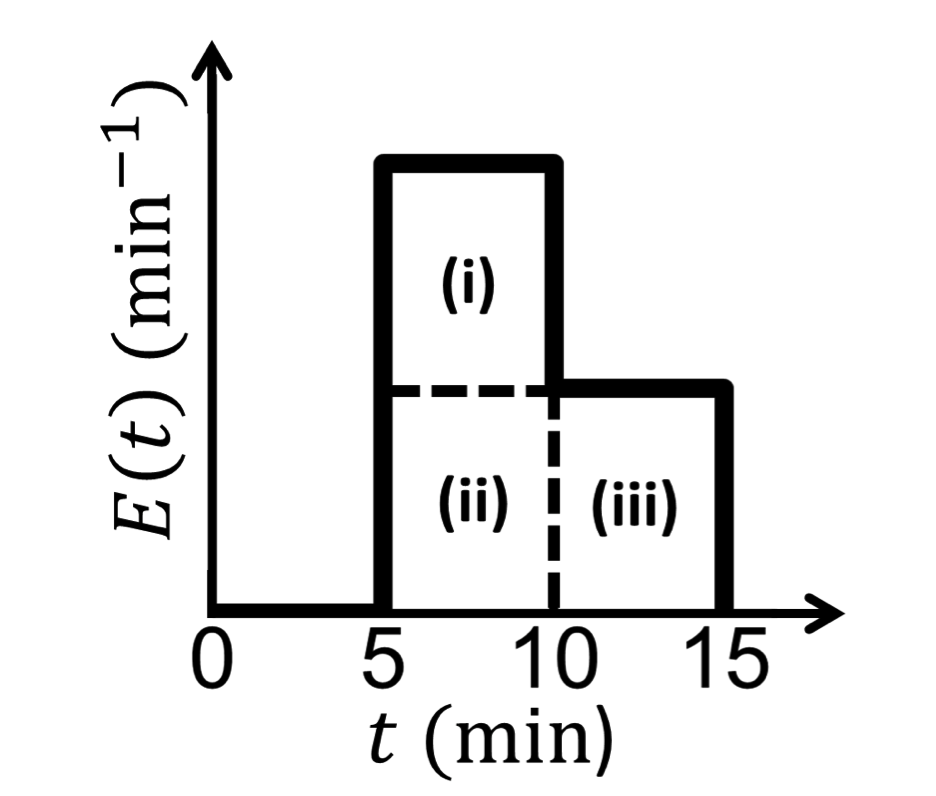
\includegraphics[width=0.5\columnwidth]{figs/60.png}
        \caption{Caption}
        \label{fig:placeholder}
    \end{figure}
    \item The outlet concentration $C_A$ of a plug flow reactor (PFR) is controlled by manipulating the inlet concentration $C_{A0}$. The following transfer function describes the dynamics of this PFR.
    \begin{align*}
       \frac{C_A\brak{s}}{C_{A0}\brak{s}} = exp\sbrak{-\frac{V}{F}\brak{k+s}}
    \end{align*}
    In the above equation, $V = 1m^3$ , $F = 0.1m^3min^{-1}$ and $k = 0.5min^{-1}$. The measurement and valve transfer functions are both equal to 1. The ultimate gain, defined as the proportional controller gain that produces sustained oscillations, for this system is \rule{40pt}{0.1mm} (rounded off to one decimal place).

    \hfill{\brak{\text{GATE CH 2023}}}
    \item The transfer function of a measuring instrument is
    \begin{align*}
        G_m\brak{s} = \frac{1.05}{2s + 1}exp\brak{-s}
    \end{align*}
    At time $t = 0$, a step change of +1 unit is introduced in the input of this instrument. The time taken by the instrument to show an increase of 1 unit in its output is \rule{30pt}{0.1mm} (rounded off to two decimal places).

    \hfill{\brak{\text{GATE CH 2023}}}
    \item A design engineer needs to purchase a membrane module (M) for a plant. Details about the two available options, M1 and M2, are given in the table below. The overall plant has an expected life of 7 years. If the interest rate is 8 \% per annum, compounded annually, the difference in the net present value (NPV) of these two options, in lakhs of rupees, is \rule{30pt}{0.1mm} (rounded off to one decimal place).

    \hfill{\brak{\text{GATE CH 2023}}}
    \begin{table}[H]
\centering
\begin{tabularx}{0.5\textwidth}{|l|X|X|}
\hline
\textbf{} & \textbf{M1} & \textbf{M2} \\
\hline
Purchase cost(in lakhs of rupees) & 10 & 5 \\
\hline
Expected life(years) & 5 & 3 \\
\hline
\end{tabularx}
\caption*{}
\end{table}
    \item The purchase cost of a new distillation column is Rs.10 lakhs with an installation factor of 5.8. The cost of the capital is to be annualized over a period of 6 years at a fixed rate of interest of 5 \% per annum, compounded annually. The annual cost (in lakhs of rupees) of the installed capital is \rule{40pt}{0.1mm}(rounded off to one decimal place).

    \hfill{\brak{\text{GATE CH 2023}}}
    \item Pumps $A$ and $B$ are being considered for purchase in a chemical plant. Cost details for these two pumps are given in the table below. The interest rate is 10 \% per annum, compounded annually. For both the pumps to have the same capitalized cost, the salvage value (in Rs.) of pump B should be \rule{30pt}{0.1mm}(rounded off to the nearest integer).

\hfill{\brak{\text{GATE CH 2023}}}
\begin{table}[H]
\centering
\begin{tabularx}{0.6\textwidth}{|l|X|X|}
\hline
\textbf{Item} & \textbf{Pump A} & \textbf{Pump B} \\
\hline
Installed cost (Rs.) & 16000 & 32000 \\
\hline
Uniform end of year maintenance (Rs.) & 2400 & 1600 \\
\hline
Salvage value (Rs.) & 1000 & ? \\
\hline
Service life (year(s)) & 1 & 2 \\
\hline
\end{tabularx}
\caption*{}
\end{table}

\section*{END OF QUESTION PAPER}














\end{enumerate}

\end{document}
